\documentclass{article}
% main document, called main.tex
\usepackage{tikz}
\usetikzlibrary{external}

\usetikzlibrary{positioning}
\usetikzlibrary{calc}
\usetikzlibrary{shapes.geometric, arrows, arrows.meta}
\usepackage{varwidth}% http://ctan.org/pkg/varwidth
\usetikzlibrary{shadows,trees, mindmap}
\usetikzlibrary{matrix}
\usetikzlibrary{fit}

\tikzexternalize % activate!
\begin{document}
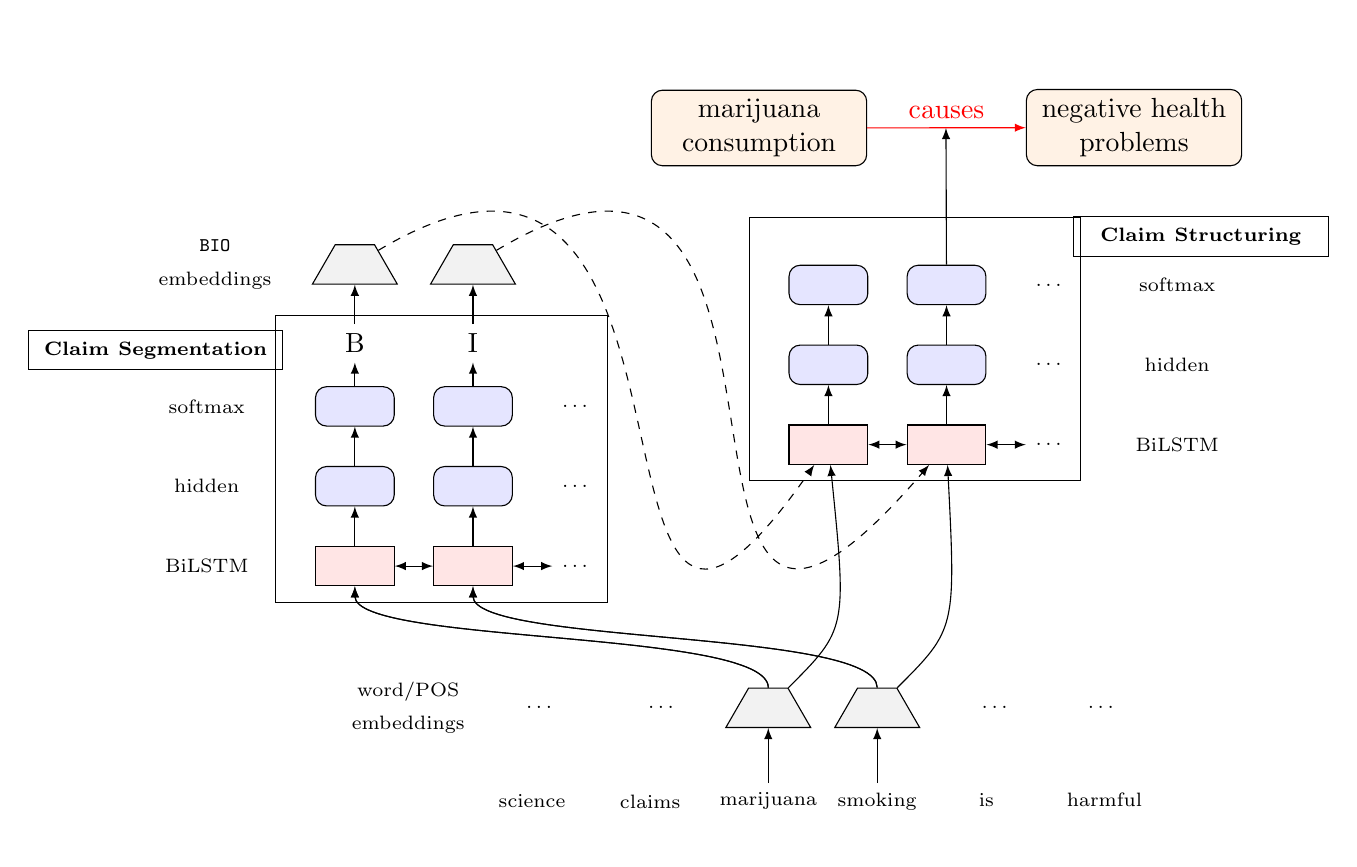
\begin{tikzpicture}[node distance=1.5cm]
\tikzstyle{lstm} = 
[rectangle, minimum width=1cm, minimum height=0.5cm, text
centered, draw=black, fill=red!10]
\tikzstyle{hidden} = 
[rectangle, minimum width=1cm, minimum height=0.5cm, text 
centered, draw=black, fill=blue!10, rounded corners]
\tikzstyle{embed} = 
[trapezium, minimum width=1cm, minimum height=0.5cm, text 
centered, draw=black, fill=gray!10]
\tikzstyle{label} = 
[minimum width=1cm, minimum height=0.5cm, text 
centered, text width=1.5cm]
\tikzstyle{dots} = 
[minimum width=0.3cm, 
minimum height=0.5cm, text 
centered, text width=0.3cm]
\tikzstyle{component} = 
[minimum width=1cm, minimum height=0.5cm, text 
centered, text width=3cm, rectangle, draw=black]
\tikzstyle{concept} =
[rectangle, minimum width=1cm, minimum height=0.5cm, text 
centered, draw=black, fill=orange!10, rounded corners, text width=2.5cm]

\node (lstm_1) [lstm] {};
\node (lstm_2) [lstm, right of=lstm_1] {};
\node (dots_1) [dots, right=0.5cm of lstm_2] {\scriptsize{\dots}};
\node (hidden_1) [hidden, above=0.5cm of lstm_1] {};
\node (hidden_2) [hidden, above=0.5cm of lstm_2] {};
\node (dots_2) [dots, right=0.5cm of hidden_2] {\scriptsize{\dots}};

\node (hidden_3) [hidden, above=0.5cm of hidden_1] {};
\node (hidden_4) [hidden, above=0.5cm of hidden_2] {};
\node (dots_3) [dots, right=0.5cm of hidden_4] {\scriptsize{\dots}};

\node (B_lab) [above=0.3cm of hidden_3] {B};
\node (I_lab) [above=0.3cm of hidden_4] {I};

\node (trapez_1) [embed, above=0.5 cm of B_lab] {};
\node (trapez_2) [embed, above=0.5 cm of I_lab] {};

\draw ($(hidden_3.north west) + (-0.5, 0.9)$) rectangle ($(lstm_2.south east) + (1.2, -0.2)$);

\node (word_1) [below right=2.5cm and 4cm of lstm_1] {\scriptsize{marijuana}};
\node (word_2) [below right=2.5cm and 4cm of lstm_2] {\scriptsize{smoking}};
\node (word_3) [right of=word_2] {\scriptsize{is\textcolor{white}{jg}}};
\node (word_4) [right of=word_3] {\scriptsize{harmful\textcolor{white}{jg}}};
% \node (word_0) [left of=word_1] {\scriptsize{\dots}};
% \node (word_5) [right of=word_4] {\scriptsize{\dots}};
\node (word_m1) [left of=word_1] {\scriptsize{claims}};
\node (word_m2) [left of=word_m1] {\scriptsize{science}};

\node (w_1) [embed, above=0.7cm of word_1] {};
\node (w_2) [embed, above=0.7cm of word_2] {};
\node (dots_word1) [dots, right=0.8cm of w_2] {\scriptsize{\dots}};
\node (dots_word4) [dots, right=0.8cm of dots_word1] {\scriptsize{\dots}};
\node (dots_word2) [dots, left=0.7cm of w_1] {\scriptsize{\dots}};
\node (dots_word3) [dots, left=1cm of dots_word2] {\scriptsize{\dots}};

\node (lstm_3) [lstm, above right=-1 cm and 3.5cm of hidden_4] {};
\node (lstm_4) [lstm, right of=lstm_3] {};
\node (hidden_5) [hidden, above=0.5cm of lstm_3] {};
\node (hidden_6) [hidden, above=0.5cm of lstm_4] {};
\node (hidden_7) [hidden, above=0.5cm of hidden_5] {};
\node (hidden_8) [hidden, above=0.5cm of hidden_6] {};
\node (lstm2_dots_1) [dots, right=0.5cm of lstm_4] {\scriptsize{\dots}};
\node (lstm2_dots_2) [dots, right=0.5cm of hidden_6] {\scriptsize{\dots}};
\node (lstm2_dots_3) [dots, right=0.5cm of hidden_8] {\scriptsize{\dots}};

%\node (struc) [above=0.8cm of hidden_8] {};
\node (c_marijuana) [concept, above left=1.25 cm and 0.5cm of hidden_8] {marijuana consumption };
\node (c_health) [concept, above right=1.25cm and 0.5cm of hidden_8] {negative health problems};
\draw[-latex] (hidden_8) -- ($(c_marijuana.east) + (1, 0) $);

\draw[-latex, red] (c_marijuana) -- (c_health) node[midway, above] {causes};

\draw ($(hidden_7.north west) + (-0.5, 0.6)$) rectangle ($(lstm_4.south east) + (1.2, -0.2)$);
%\draw ($(hidden_7.north west) + (-0.3, 0.6)$) rectangle ($(lstm_4.south east) + (0.3, -0.6)$);
% 
% \node (lstm_5) [lstm, right=1 cm of lstm_4] {};
% \node (lstm_6) [lstm, right of=lstm_5] {};
% \node (hidden_9) [hidden, above=0.5cm of lstm_5] {};
% \node (hidden_10) [hidden, above=0.5cm of lstm_6] {};
% \node (hidden_11) [hidden, above=0.5cm of hidden_9] {};
% \node (hidden_12) [hidden, above=0.5cm of hidden_10] {};
% 
% \draw ($(hidden_11.north west) + (-0.3, 0.6)$) rectangle ($(lstm_6.south east) + (0.3, -0.6)$);
% 
% \node (lstm_7) [lstm, right=1 cm of lstm_6] {};
% \node (lstm_8) [lstm, right of=lstm_7] {};
% \node (hidden_13) [hidden, above=0.5cm of lstm_7   ] {};
% \node (hidden_14) [hidden, above=0.5cm of lstm_8   ] {};
% \node (hidden_15) [hidden, above=0.5cm of hidden_13] {};
% \node (hidden_16) [hidden, above=0.5cm of hidden_14] {};
% 
% \draw ($(hidden_15.north west) + (-0.3, 0.6)$) rectangle ($(lstm_8.south east) + (0.3, -0.6)$);

% labels of NN parts
\node (label_word_pos) [label, left=0.5cm of dots_word3] {\scriptsize{word/POS embeddings}};
\node (label_bilstm1) [label, left=0.5cm of lstm_1] {\scriptsize{BiLSTM}};
\node (label_hidden1) [label, left=0.5cm of hidden_1] {\scriptsize{hidden}};
\node (label_softmax1) [label, left=0.5cm of hidden_3] {\scriptsize{softmax}};
\node (bio_embeddings) [label, left=0.5cm of trapez_1] {\scriptsize{\texttt{BIO} embeddings}};

\node (label_bilstm1) [label, right=0.5cm of lstm2_dots_1] {\scriptsize{BiLSTM}};
\node (label_hidden1) [label, right=0.5cm of lstm2_dots_2] {\scriptsize{hidden}};
\node (label_softmax1) [label, right=0.5cm of lstm2_dots_3] {\scriptsize{softmax}};

%\node (label_bilstm2) [label, left=0.5cm of lstm_3] {\scriptsize{BiLSTM}};
%\node (label_hidden2) [label, left=0.5cm of hidden_] {\scriptsize{hidden}};
%\node (label_softmax2) [label, left=0.5cm of hidden_3] {\scriptsize{softmax}};

\node (bio_lstm) [component, above left=0.2cm and 0.4cm of hidden_3] 
{\scriptsize{\textbf{Claim Segmentation}}};

\node (struc_lstm) [component, above right=0.1cm and 1.1cm of hidden_8] 
{\scriptsize{\textbf{Claim Structuring}}};

%text width=4cm,minimum height=6cm,minimum width=10cm

% connections
% \draw[-latex] (trapez_1) .. controls +(up:1.5cm) and +(down:1cm) ..
% node[above, sloped] {} (lstm_3);
% \draw[-latex] (trapez_2) .. controls +(up:1.5cm) and +(down:1cm) ..
% node[above, sloped] {} (lstm_4);
% 
% \draw[-latex] (trapez_1) .. controls +(up:1.3cm) and +(down:2cm) ..
% node[above, sloped] {} (lstm_5);
% \draw[-latex] (trapez_2) .. controls +(up:1.3cm) and +(down:2.5cm) ..
% node[above, sloped] {} (lstm_6);
% 
% \draw[-latex] (trapez_1) .. controls +(up:1cm) and +(down:3cm) ..
% node[above, sloped] {} (lstm_7);
% \draw[-latex] (trapez_2) .. controls +(up:1cm) and +(down:3.5cm) ..
% node[above, sloped] {} (lstm_8);

% lstm connections
\draw[-latex] (lstm_1) -- (hidden_1);
\draw[-latex] (lstm_2) -- (hidden_2);
\draw[-latex] (hidden_1) -- (hidden_3);
\draw[-latex] (hidden_2) -- (hidden_4);
\draw[-latex] (hidden_3) -- (B_lab);
\draw[-latex] (hidden_4) -- (I_lab);

%\draw[-latex] (hidden_8) -- (struc);

% \draw[-latex] (lstm_1) .. controls +(up:1.1cm) and +(left:0.9cm) .. node[above, sloped] {} (lstm_2);
% \draw[-latex] (lstm_2) .. controls +(up:1.1cm) and +(left:0.7cm) .. node[above, sloped] {} (dots_1);

\draw[>=latex, <->] (lstm_1) -- (lstm_2);
\draw[>=latex, <->] (lstm_2) -- (dots_1);

\draw[>=latex, <->] (lstm_3) -- (lstm_4);
\draw[>=latex, <->] (lstm_4) -- (lstm2_dots_1);

\draw[-latex, dashed] (trapez_1) .. controls +(5cm, 3cm) and +(-3.5cm, -5cm) .. node[above, sloped] {} (lstm_3);
\draw[-latex, dashed] (trapez_2) .. controls +(5cm, 3cm) and +(-4.3cm, -5cm) .. node[above, sloped] {} (lstm_4);

\draw[-latex] (w_1) .. controls +(up:1cm) and +(down:1cm) .. node[above, sloped] {} (lstm_1);
\draw[-latex] (w_2) .. controls +(up:1cm) and +(down:1cm) .. node[above, sloped] {} (lstm_2);

\draw[-latex] (w_1) .. controls +(up:1cm) and +(down:1cm) .. node[above, sloped] {} (lstm_1);
\draw[-latex] (w_2) .. controls +(up:1cm) and +(down:1cm) .. node[above, sloped] {} (lstm_2);

\draw[-latex] (w_1) .. controls +(1cm, 1cm) .. node[above, sloped] {} (lstm_3);
\draw[-latex] (w_2) .. controls +(1cm, 1cm) .. node[above, sloped] {} (lstm_4);

%\draw[-latex] (w_1) -- (lstm_1);
%\draw[-latex] (w_2) -- (lstm_2);
\draw[-latex] (word_1) -- (w_1);
\draw[-latex] (word_2) -- (w_2);
\draw[-latex] (B_lab) -- (trapez_1);
\draw[-latex] (I_lab) -- (trapez_2);

\draw[-latex] (lstm_3) -- (hidden_5);
\draw[-latex] (lstm_4) -- (hidden_6);
\draw[-latex] (hidden_5) -- (hidden_7);
\draw[-latex] (hidden_6) -- (hidden_8);

\end{tikzpicture}

\end{document}


